\section{Results and Discussions}
\label{sec:results}

\begin{figure*}
	\centering
	\textbf{\em  4-class pair-level results. \quad\quad \quad            6-class pair-level results.    \quad      \quad\quad    13-class pair-level results}\vspace{-1.0cm}\\
	\subfigure{
		\begin{minipage}{0.25\linewidth}
			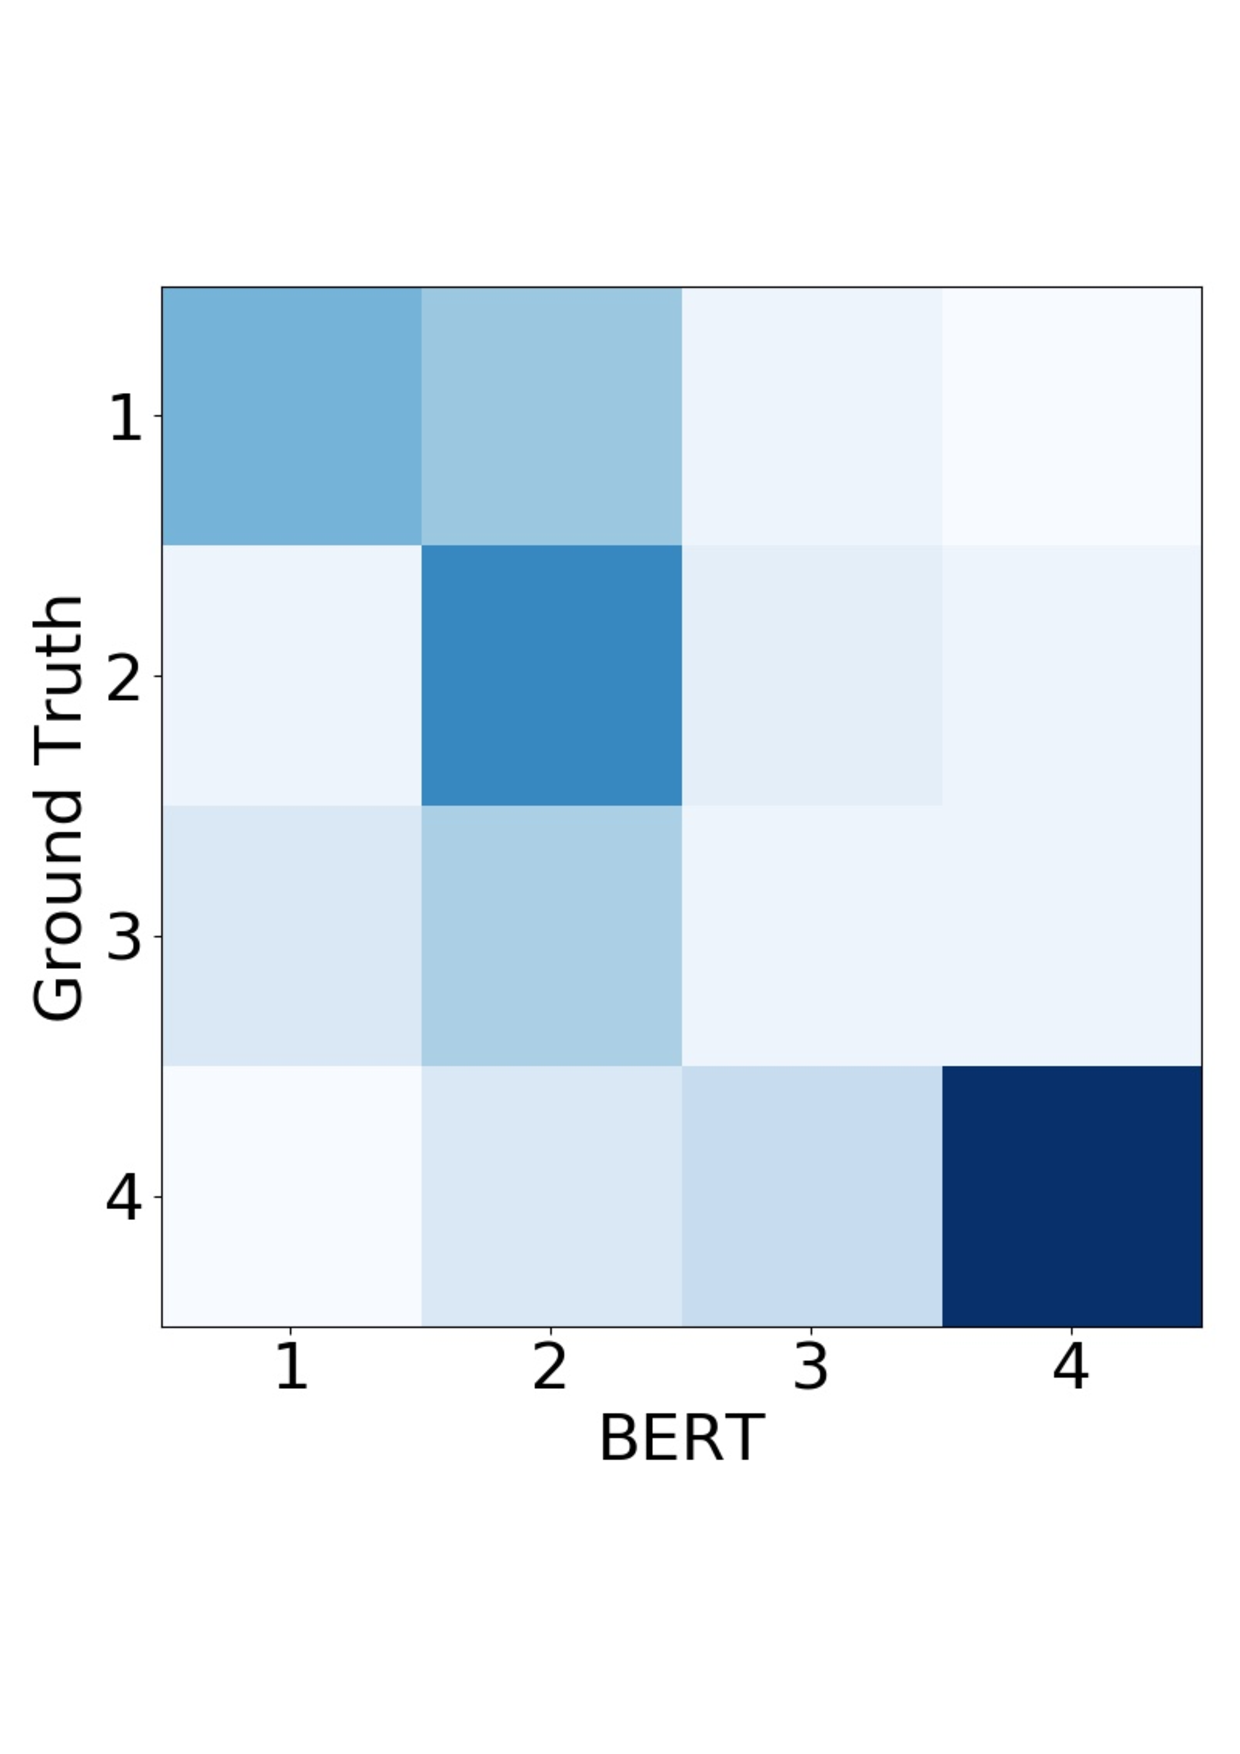
\includegraphics[width=1\linewidth]{BERT_4_pair}\vspace{-1.75cm}
			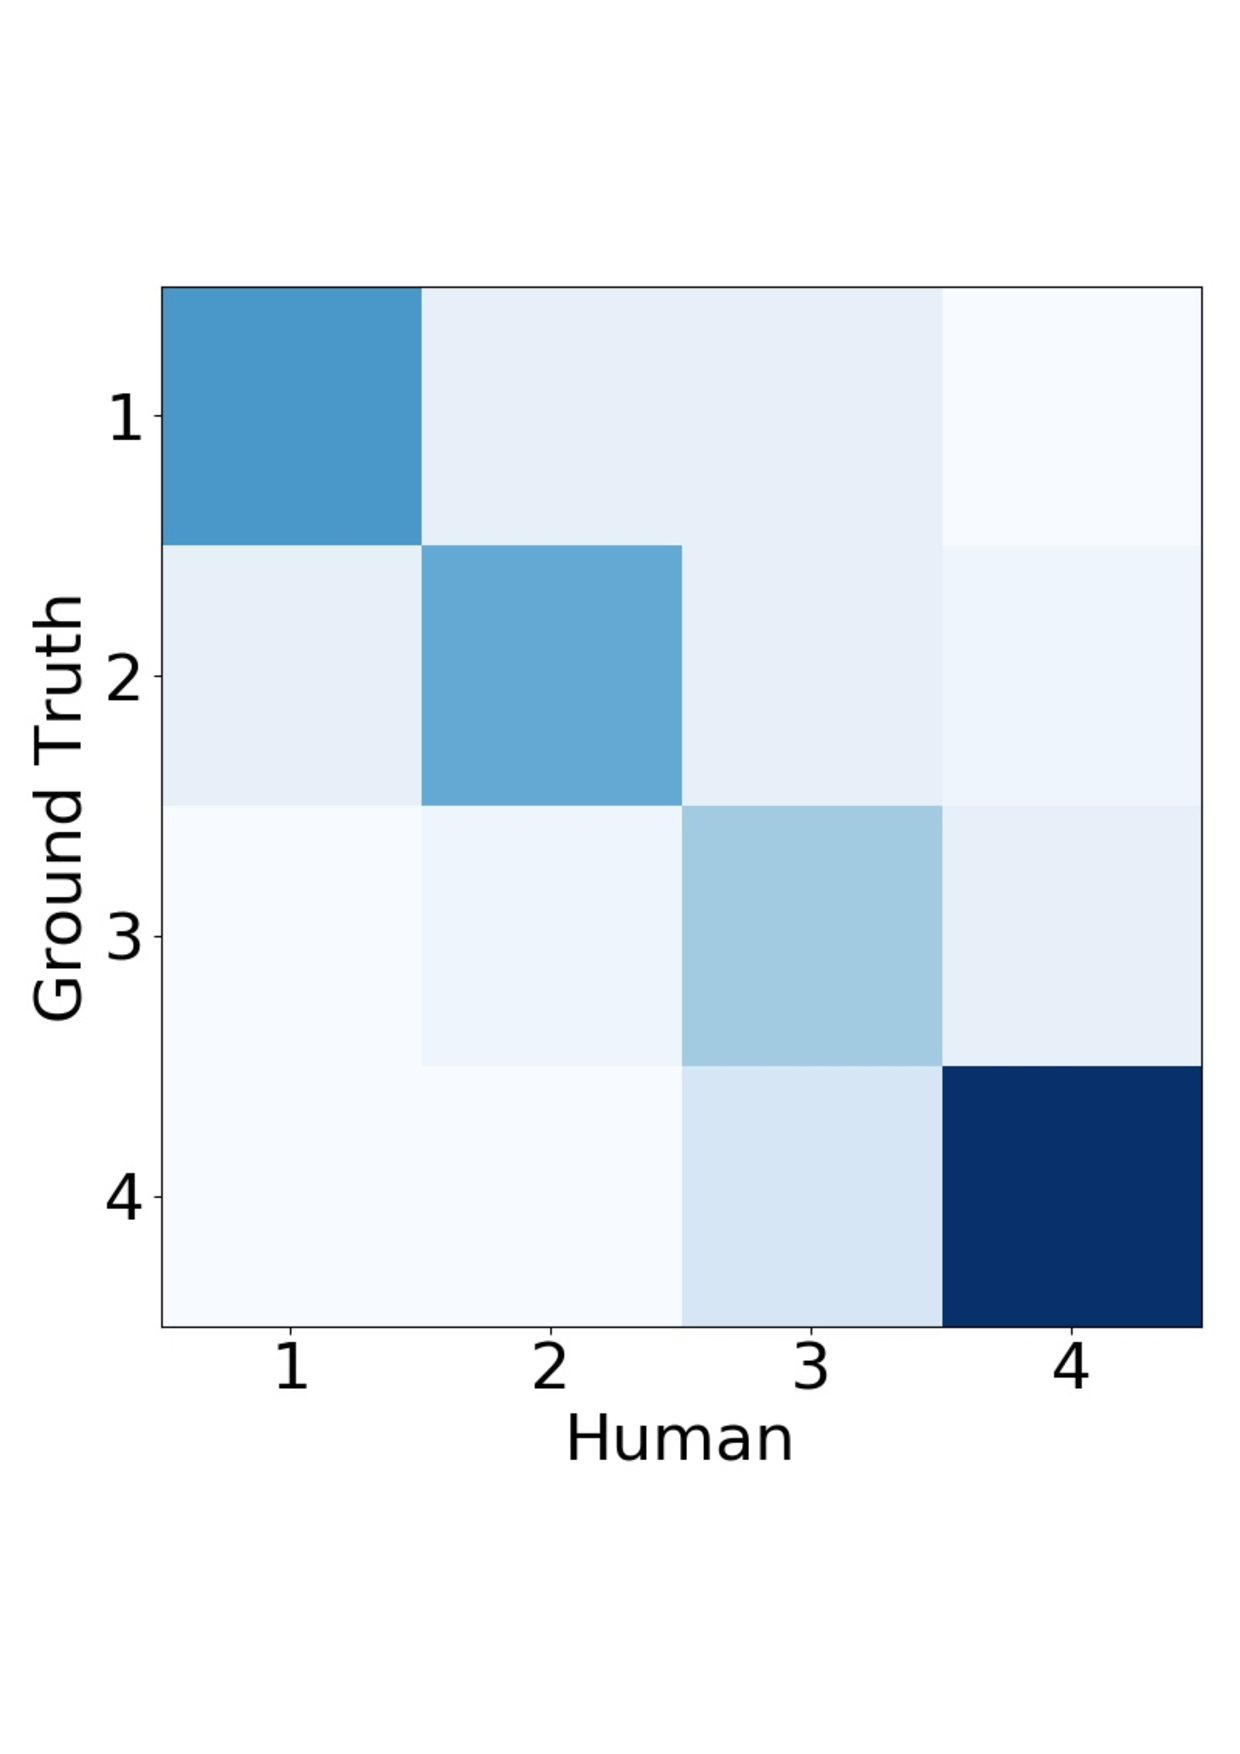
\includegraphics[width=1\linewidth]{human_4_pair}
	\end{minipage}}
	\subfigure{
		\begin{minipage}{0.25\linewidth}
			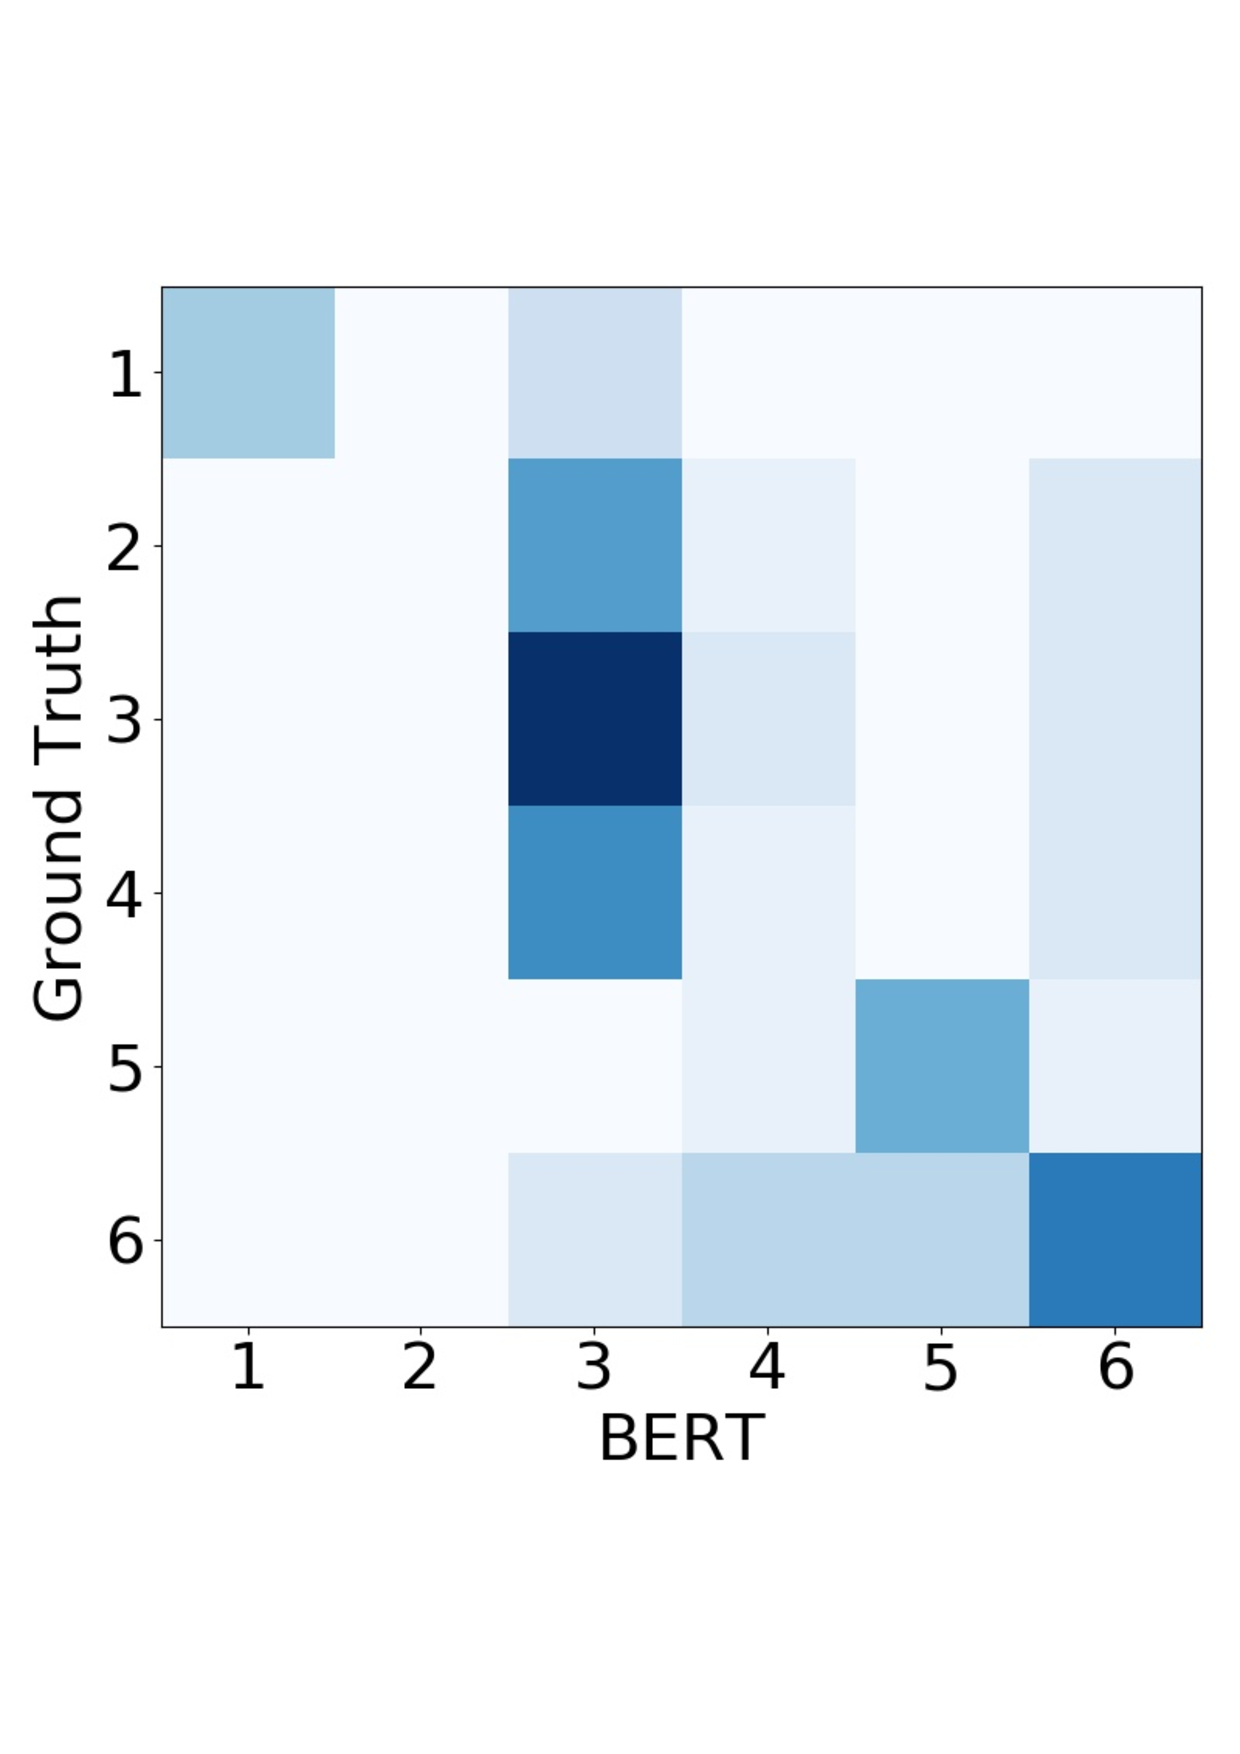
\includegraphics[width=1\linewidth]{BERT_6_pair}\vspace{-1.75cm}
			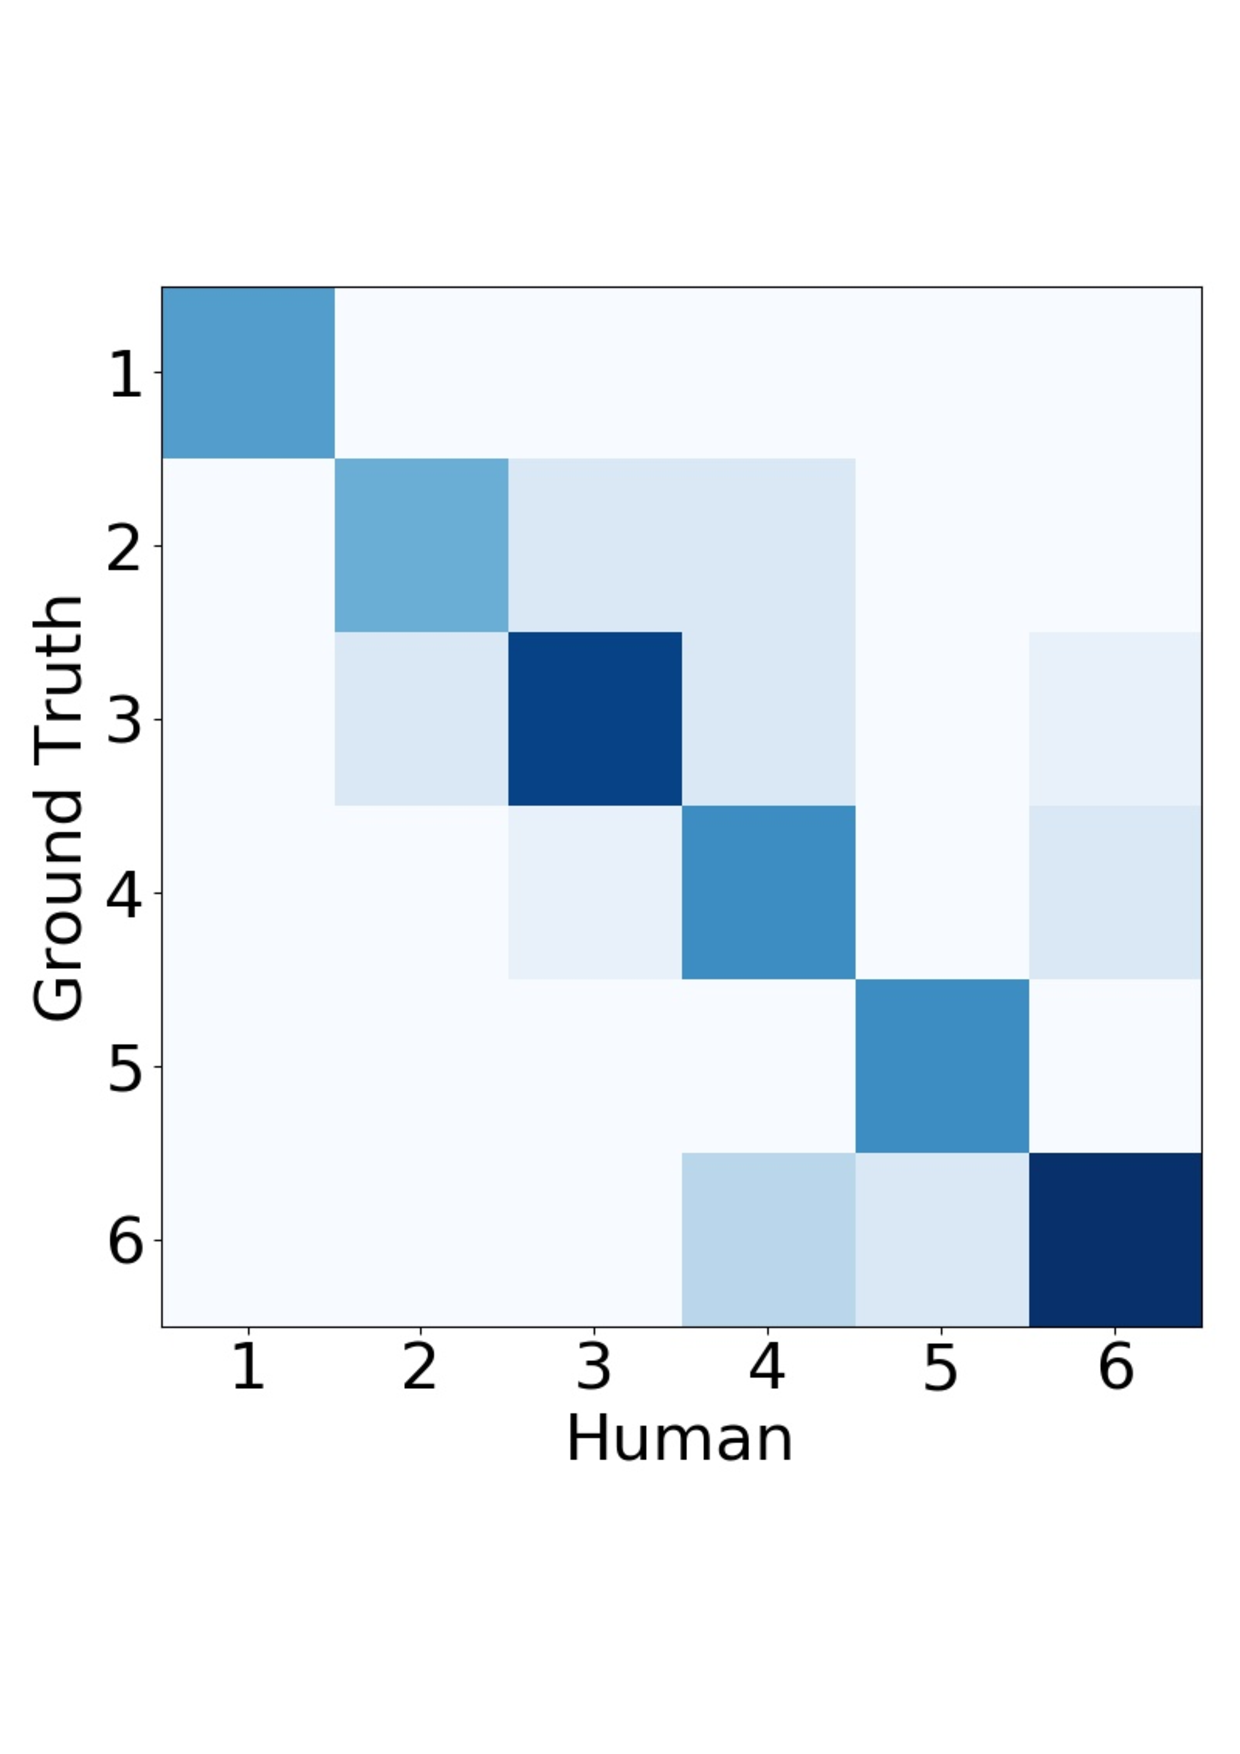
\includegraphics[width=1\linewidth]{human_6_pair}
	\end{minipage}}
	\subfigure{
		\begin{minipage}{0.25\linewidth}
			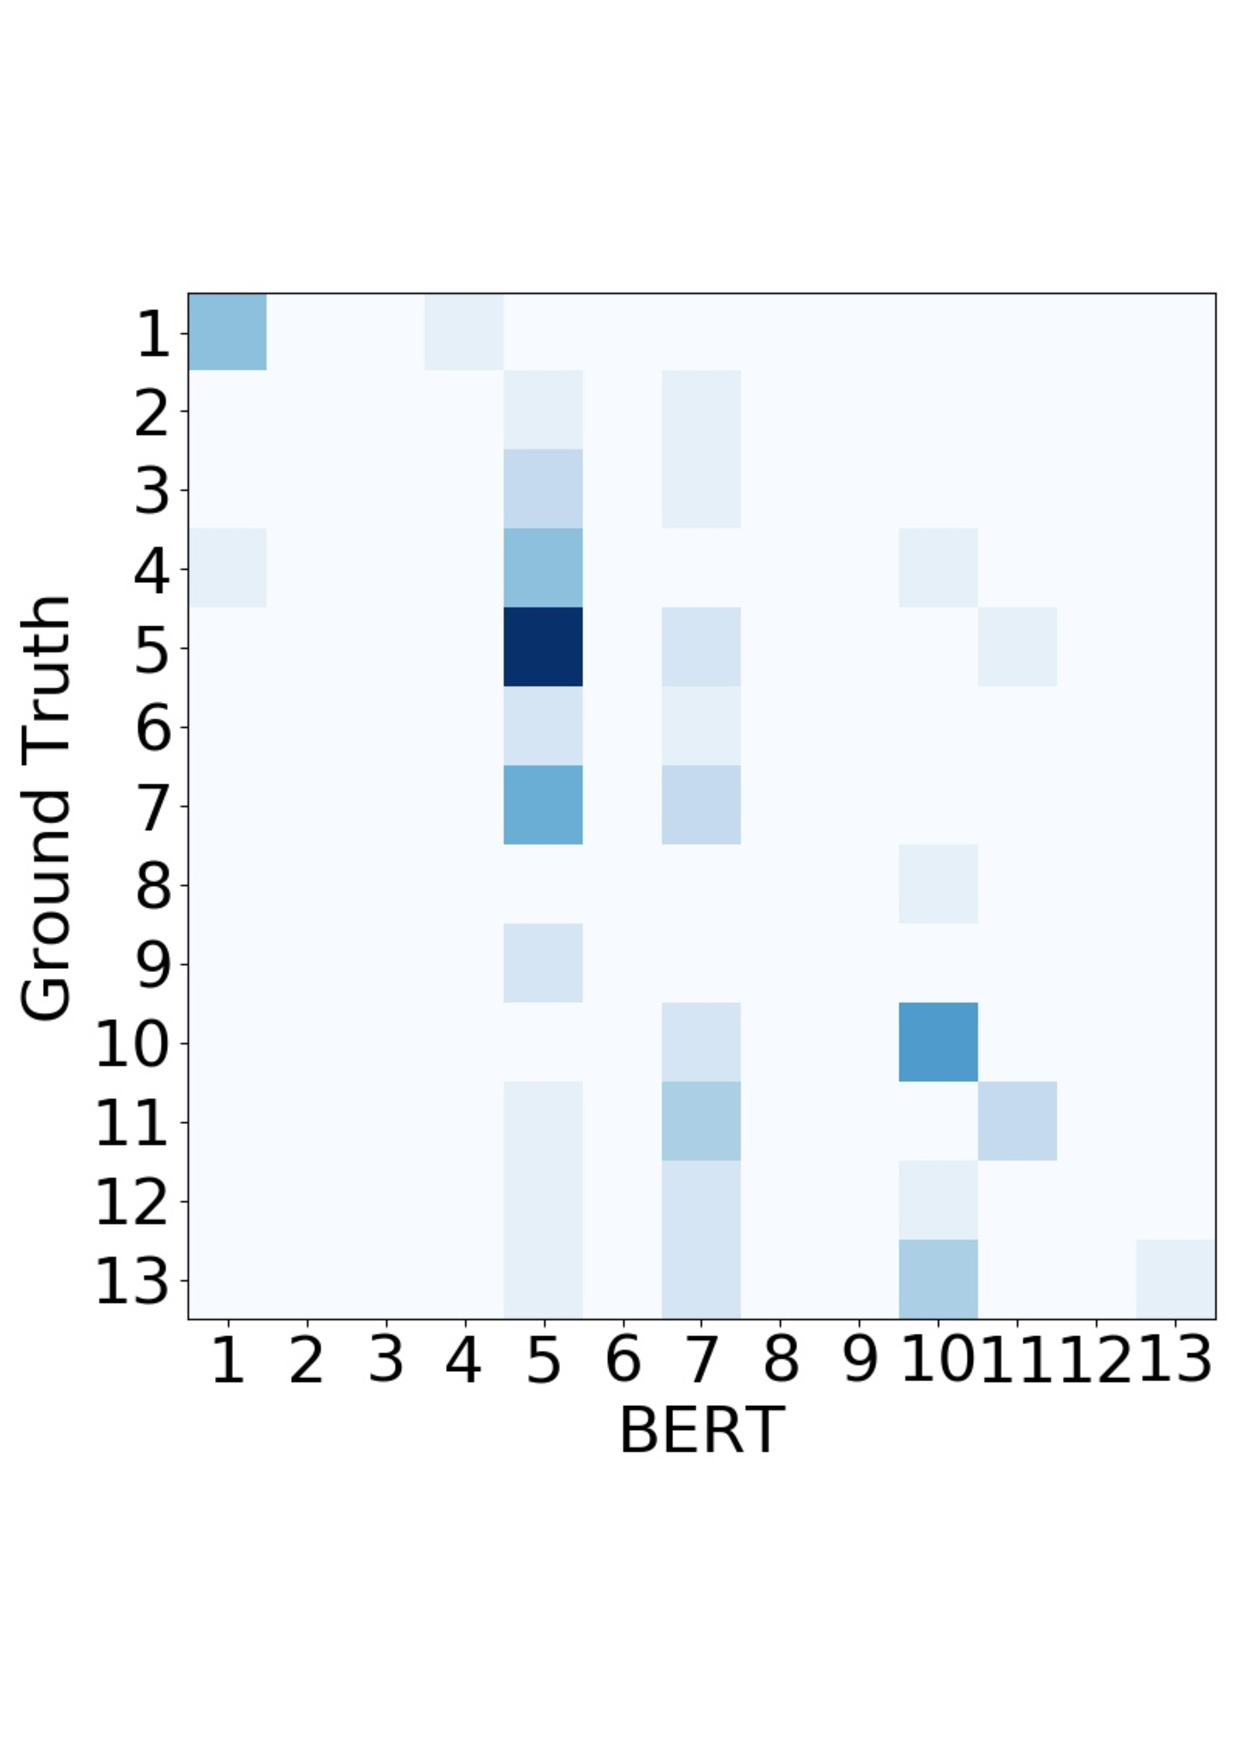
\includegraphics[width=1\linewidth]{BERT_13_pair}\vspace{-1.75cm}
			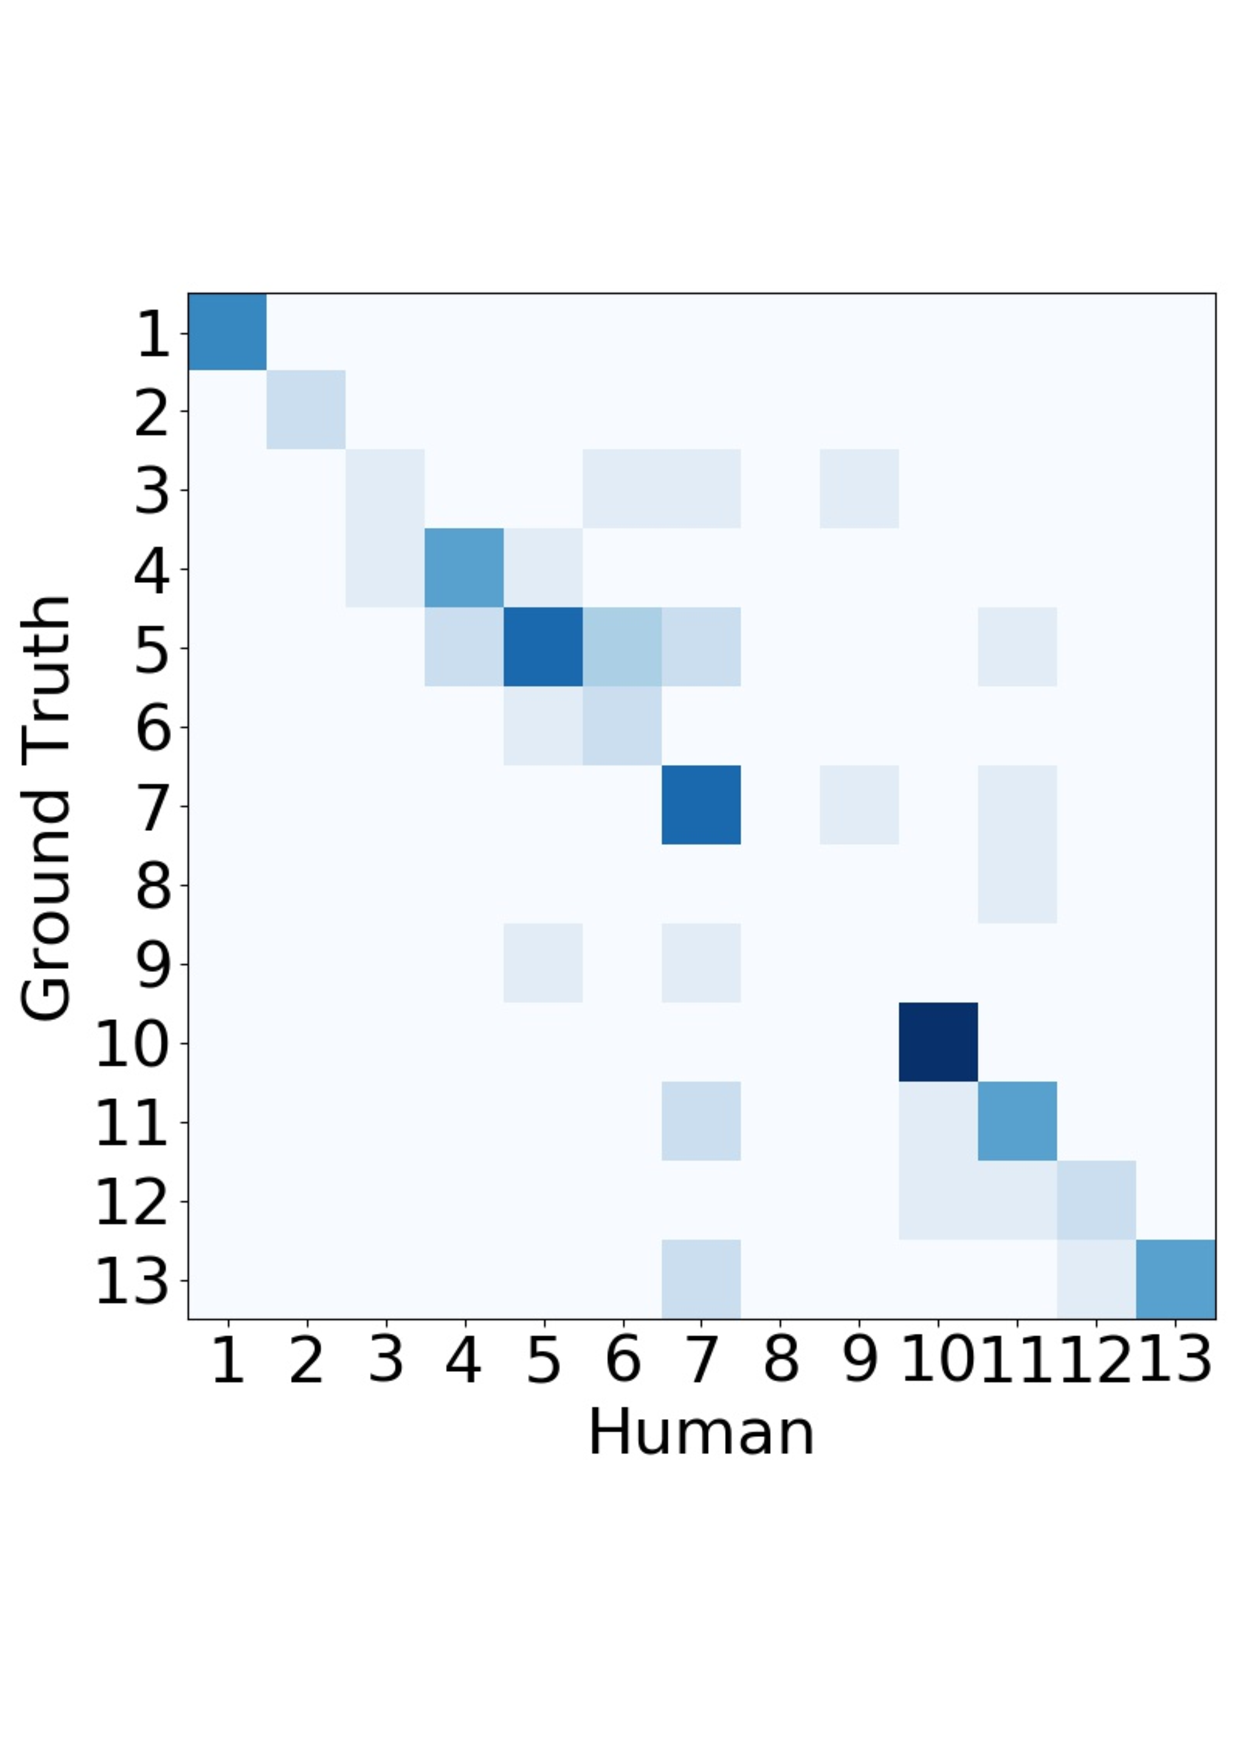
\includegraphics[width=1\linewidth]{human_13_pair}
	\end{minipage}}
	\vspace{-1cm}
	\caption{The confusion matrix of relation classification tasks.}
	\label{fig:confusion}
\end{figure*}
In this section, we discussed the classification performances and a simple data augmentation method for pair-level classification with a case study and future directions.
\subsection{Session-level Performance}
We run all of the baseline models with three different random seeds and then obtain the mean and
std value of the evaluation metrics. The results of baselines and human upper bound on session-level relation classification task 
are shown in Table \ref{tab:results}. The difficulties on session-level tasks is in proportional to the number of classes, as the performances of all of the models and human annotators decrease from 4-class task to 13-class task. The gap is about 10\% and 20\% on accuracy for models and human evaluation respectively. 

For Majority, the accuracy is even higher than a neural baseline (LSTM), while the F1-macro is the lowest due to the unbalanced data distribution between classes. The neural baselines mostly performs better than Random and Majority.

The comparison of performances on neural baselines is BERT$>$CNN$>$LSTM. LSTM is much weaker than CNN. The gap between them on 13-class classification is smaller than 4-class and 6-class classifications due to the fact them both of them failed on fine-grained classification task. The F1-macro is only 4.63\% and 9.20\% respectively with high variance.
BERT, a pre-trained language model baseline, performs much better and stable than the other two neural models with higher scores and lower variance. The gaps between evaluation metrics are also smaller than other baselines, indicating that it can handle the problem of imbalanced data to some extent.

The human performance is the average score of two annotators. We calculate the Cohen's Kappa between them, and the agreement are 0.429, 0.336 and 0.301 for 4-class, 6-class and 13-class relation classification tasks respectively. The agreement on 6-class and 13-class tasks are fair, and on more coarse-grained task, 4-class task, is moderate. It' s also quite difficult for human to identifying the relationship between interlocutors based on only one session. It seems that BERT outperforms human upper bound on accuracy of the 13-class classification task, but actually there is no significant differences between them, and F1-macro score of human upper bound is statistically significantly better than BERT with p-value less than 0.05.



\subsection{Pair-level Performance}

\label{sec:pair}
Table \ref{tab:results} also included the results on pair-level tasks. The difficulties between classification tasks on different granularity are the same as session-level classification tasks and the comparisons between baseline models are also the same: BERT$>$CNN$>$LSTM. 

By using the MRR metric to get the prediction on pair-level performance of each model as explained in Section \ref{sec:baselines}, it aggravate the polarization of the model performances. The strong baselines like CNN (except on 13-class classification task) and BERT achieve higher scores on pair-level tasks, while others, including LSTM and 13-class CNN model, performs even worse on pair-level tasks. The performance of LSTM is close to Majority baseline. The reason for this phenomenon is that we only assign one label for multiple sessions on pair-level tasks. If the model is weak, it tends to give some extremely unreasonable predictions on some of the sessions for a given pair of interlocutors. Even though there may be some correct predictions on session level, the final prediction for this pair is wrong. On the other hand, if the model is strong, it can give more reasonable predictions for most sessions. Then although there may be some wrong cases on session level, they will be tolerated. The performance of these models will increase.

The gap between CNN and BERT decreases from 4-class to 6-class tasks while increases greatly from 6-class to 13-class tasks. The convolution-based model seems more stable on coarse-grained tasks, and drops dramatically on the 13-class fine-grained task. On the contrary, the performance of fine-tuned language model decreases rapidly from 4-class to 6-class tasks and decreases slowly from 6-class to 13-class tasks. As a result, the advantage of BERT model on 6-class classification tasks is limited beyond the CNN baseline.

Human annotators also performance much better on pair-level tasks than session-level tasks. The Cohen's Kappa for two annotators are 0.698, 0.687 and 0.614 for 4-class, 6-class and 13-class classification tasks respectively, showing substantial agreements. The higher performances and agreement is consistent with the intuition that, with multiple sessions for a given pair, human are able to find more correlations between sessions and better understand the background of two interlocutors. In this way, we think pair-level relation classification tasks are more reasonable, challenging and meaningful for the development of current models. 

The gap between best baseline BERT and Human performances also showing the limitation of current models. We draw the confusion metrics for the best neural model BERT and human performances in Figure \ref{fig:confusion}. We can see that for coarse-level relation classification tasks, the performance of BERT and human has some similarities. They both did well on predicting the official relation type on 4-level task, and intimacy-peer relation type and official-peer relation type on 6-level task. For 13-classification tasks, BERT fails dramatically which may due to the unbalanced data distribution, tending to predict the relation type of ``{\em lovers}'', while human performance well on the relation type of ``{\em Workplace Superior-Subordinate}''.

\subsection{A First Step on Cross-session Consideration}
\label{sec:cross}

For the pair-level classification tasks, our neural baselines give the final predictions by aggregating the predictions for each session. In this way, some interactions between sessions may be omitted. To clarify the existence of cross-session interaction in our RRDel dataset, we augment the original pair-level samples with multiple sessions as follows: i) Cut the session into $K$ pieces according to its length (the number of utterances). ii) Concatenate the session pieces at the same cut point in two consecutive sessions to generate a new session for the given pair. It should be noted that the order of sessions in each pair follows the chronological order. For example, in Figure \ref{fig:augment} is a pair with two sessions. Each session is cut into 3 pieces when $K=3$ and we get two augmented sessions for this pair.
\begin{figure}[t!]
	\centering
	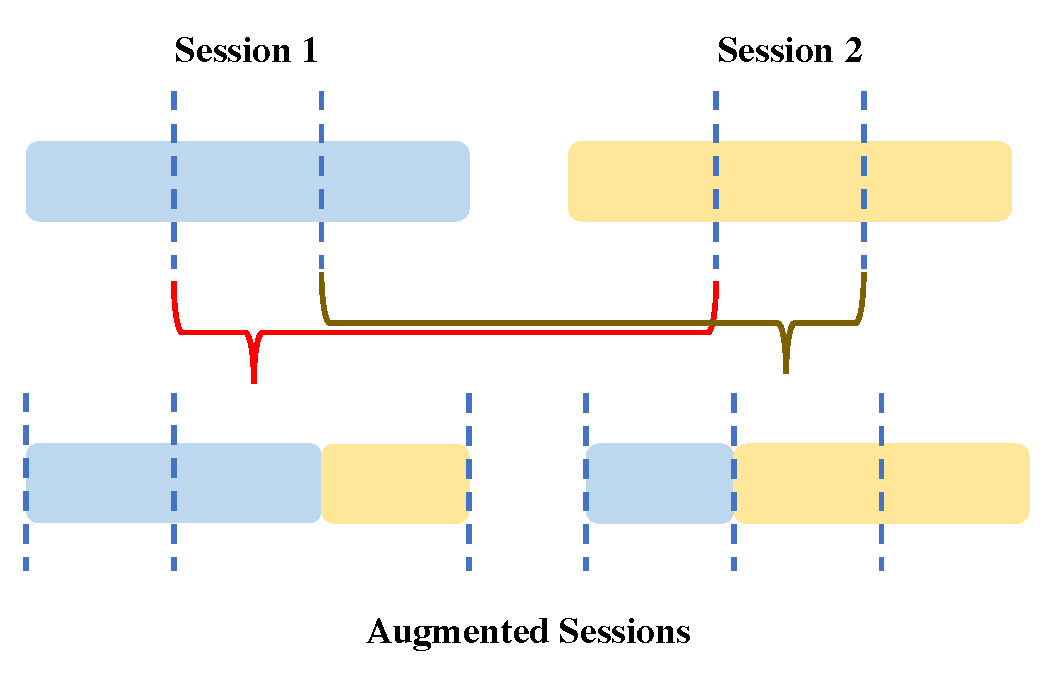
\includegraphics[width=0.7\columnwidth]{augment.pdf}
	\caption{An illustration of data augmentation when $K=3$. }
	\label{fig:augment}
\end{figure}


\begin{table}[th]
	\centering
	\scriptsize
	\begin{tabular}{@{}lcccccc@{}}
		\toprule[1.5pt]
		& \multicolumn{2}{c}{\textbf{4-class}} & \multicolumn{2}{c}{\textbf{6-class}} & \multicolumn{2}{c}{\textbf{13-class}} \\ 
		& Acc & F1-macro                 & Acc & F1-macro                  & Acc & F1-macro \\
		\midrule
		%BERT   &57.70$\pm$1.30 &50.17$\pm$1.33 & 44.87$\pm$2.55&42.27$\pm$1.29 &35.90$\pm$3.80 &19.37$\pm$2.80 \\
		$K=2$   &+1.73 &+2.50  &-0.40& -0.97& +2.13 & +0.63 \\		
		$K=3$    &+0.43 &+1.33 &+1.70 &+0.20 &+2.13 &+0.80 \\
		$K=4$    &-0.43 &+0.43 &+2.56 &+1.43 &+2.13 &+0.90 \\
		\bottomrule[1.5pt]
		
	\end{tabular}
	\caption{The pair-level classification results(\%) with data augmentation on the test set compared with BERT baseline. $K$ is the hyper-parameter for our proposed data augmentation method.}
	\label{tab:cross}
\end{table}

Using the best BERT model we trained above, we augmented the test set and re-evaluate the pair-level prediction results in Table \ref{tab:cross}. Most classification results are increased by augmentation operation. We further augmented all of the datasets in DDRel, and train and test the BERT baseline on the augmented dataset with $K=3$. The results on 6-class and 13-class enhanced significantly with accuracy equaling $49.13\%$ and $41.87\%$ respectively, and with F1-macro equaling $46.93\%$  and $26.83\%$ respectively. All of the results indicate the existence and importance of cross-session information for pair-level relationship classifications.




\subsection{Case Study and Future Directions}
We show a representative pair-level classification case with 4 sessions in Figure \ref{fig:case}. As for human, we can make inferences according to keywords 
such as ``enjoyed your sets'', ``cut a whole album'' and ``screening room''. Based on our background experience and knowledge, such conversations are more likely happening between two guys with cooperation in making music. The cues here are not obvious in single sessions but are very assuring when four sessions are considered together. Human choose ``Official'' while the best baseline BERT mistakes it to be ``Intimacy'' for this sample. The model may be confused by the informal expressions and emotional words such as ``wonderful''.


\begin{figure}[t!]
	\centering
	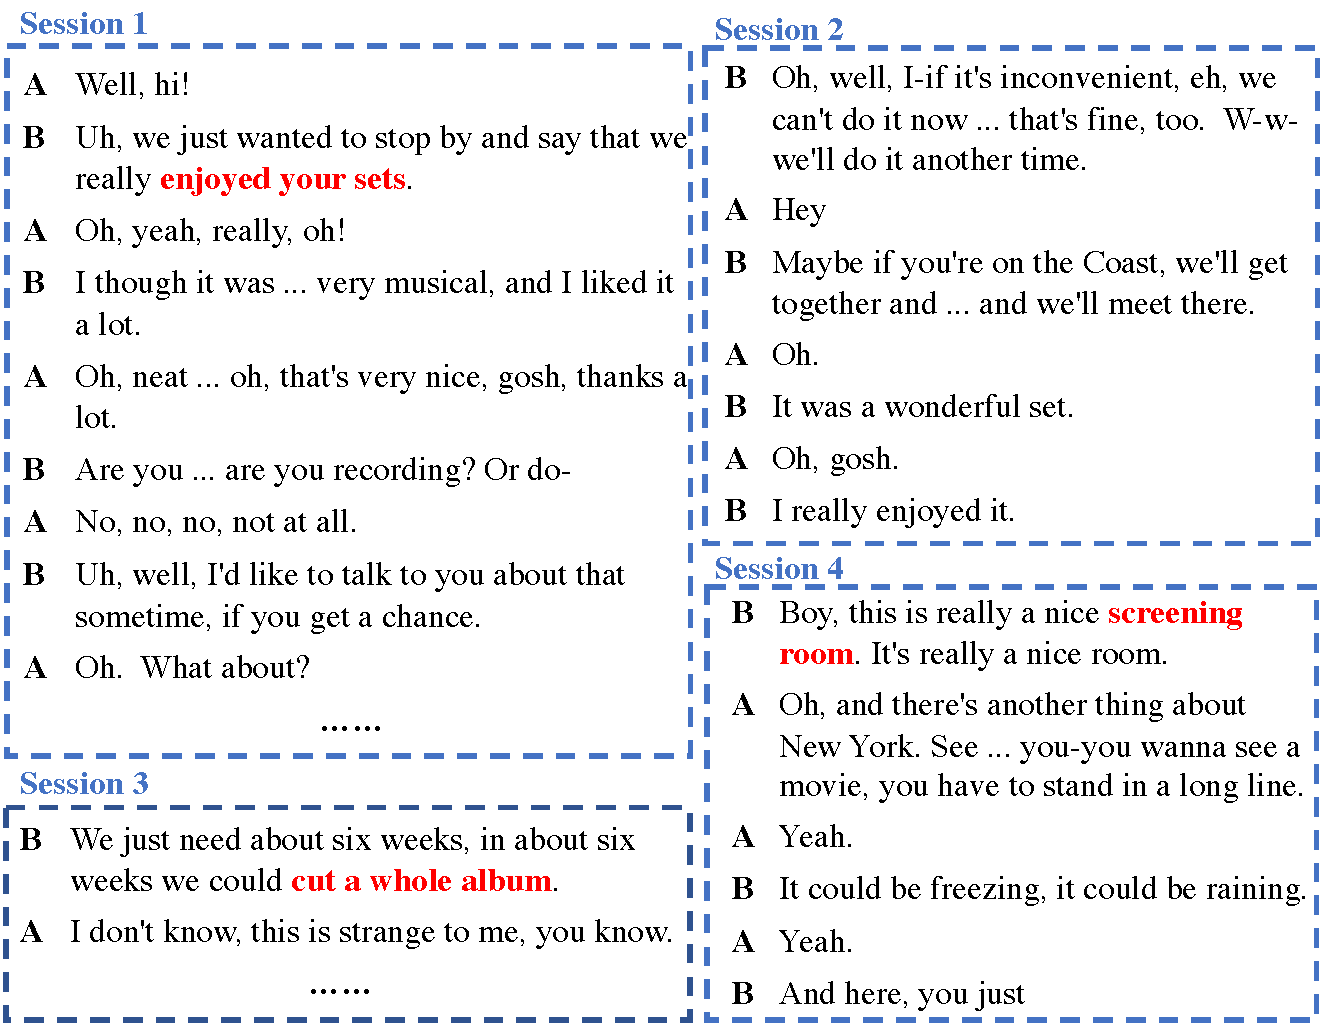
\includegraphics[width=1.0\columnwidth]{casestudy.pdf}
	\caption{A pair-level case with 4 sessions. The words colored in red are possible classification cues. }
	\label{fig:case}
\end{figure}

According to the case study, we consider the further research on this task as follows:

\textbf{Cross-session Consideration.} As talked about in Section \ref{sec:pair}, classification of a pair of interlocutors based on multiple sessions between them is a more reasonable and meaningful task. Due to the fact that the number of sessions for pairs varies a lot and it's difficult and unreasonable to concatenate all of the utterances in these sessions as the input for models, we only combines the prediction results of each session to get the final pair-level predictions and made a simple step on cross-session consideration by data augmentation. Developing models that could better find the cues between sessions is an important direction for current models.

\textbf{Commonsense Knowledge.} Another limitation of current models is due to the lack of commonsense knowledge, even for commonly pre-trained language models. Human can better inference the background of two interlocutors with the previous stories or experiences they have had. Further pre-training the language models on more similar corpus and incorporating the commonsense knowledge base, such as ConceptNet~\cite{SpeerCH17}, are possible solutions.
